\subsection{Monopole Antenna}\label{sec:monopole}
\subsubsection{Setup}
\FloatBarrier

\begin{figure}[htbp]
	\centering
	\hspace*{-0.0cm}
	\begin{subfigure}[t]{0.48\textwidth}
		\centering
		\includegraphics[height=8cm]{content/img/monopole_near_field}
		\caption{Electric near-field intensity}
		\label{fig:monopolenearfield}		
	\end{subfigure}
	\hfill
	\begin{subfigure}[t]{0.48\textwidth}
		
		\centering
		\raisebox{0.1cm}{\includegraphics[height=8cm]{content/img/monopole_antenna}}
		\caption{Geometry of monopole antenna}
		\label{fig:monopoleantenna}
	\end{subfigure}
	
	\caption{The geometrical aspects of the cylindrical monopole antenna, as implemented in the simulation model, with the respective electric near-field plot.}
	\label{fig:field_monopole_antenna}
\end{figure}

The monopole antenna is the simplest antenna capable of generating an electric dipole moment, and is therefore analyzed first to isolate this radiation mechanism. As shown in \autoref{fig:monopoleantenna}, it is installed inside the TEM cell and connected to a feed point on the top wall. The current flowing through the antenna is aligned with the electric field of the TEM mode, thereby producing an electric dipole moment according to \eqref{eqn:e_int_a} and \eqref{eqn:e_int_b}, which are further investigated in \cref{sec:eq_dip_mon}.

The antenna has a physical length of 5\,mm, making it electrically short across the entire frequency range of interest (up to 6\,GHz). Below 1.25\,GHz, the antenna is well approximated as an infinitesimal electric dipole, as discussed in \cref{sec:infinitesimal_electric_dipoles}. At higher frequencies, up to 6,GHz, the finite current distribution along the wire becomes non-negligible, and the antenna is instead treated as a small electric dipole, as described in \cref{sec:small_electric_dipole}.

Numerically, the near-field distribution exhibits strong displacement currents near the feed point and at the antenna tip. To accurately resolve these localized field concentrations, the mesh element size is reduced in both regions.

Because the electric dipole moment dominates the radiation mechanism, power transfer to the output ports occurs exclusively through displacement current coupling to the septum, as demonstrated in \cref{sec:el_small_antennas}. The induced septum current is analyzed in \cref{sec:eq_dip_mon} for two cases, including the propagation of the TEM mode alone, and exclusive propagation of the TE\textsubscript{01} mode.

As an open-circuit structure, the monopole antenna exhibits capacitive behavior. Its effect on the frequency dependence of the feed voltage, current, and input impedance is discussed in \cref{sec:v_c_z_mon}. The output power produced by the antenna is compared against that of the equivalent dipole moments in \cref{sec:output_power_mon} to validate the simulation models.

Lastly, the theoretical framework and numerical results established in this thesis are combined in \cref{sec:monopole_eqc} to construct an equivalent circuit model. The circuit model provides an analytical description and deeper understanding of the driving coupling mechanisms between the TEM cell and the monopole antenna.

\subsubsection{Equivalent dipole moments}\label{sec:eq_dip_mon}

The corresponding equivalent electric and magnetic dipole moments, $\mathbf{m}_e$ and $\mathbf{m}_m$, are analytically derived using \crefrange{eqn:ifa_me}{eqn:ifa_mm}. The resulting $\mathbf{m}_e$ shown in \autoref{fig:dipolemomentsmonopolewide} increases approximately linearly over frequency, while the magnetic dipole moment is negligible over the whole frequency range. 

Furthermore, the phase difference between the power at the two output ports is zero across the entire frequency range. This observation is consistent with the assumption that a pure electric dipole moment introduces no phase shift between the output port powers, as discussed in \autoref{sec:equ-dip-mom}.


\begin{figure}[htbp]
	\centering
	\includegraphics[width=1\linewidth]{content/img/dipole_moments_monopole_wide}
	\caption{The equivalent electric and magnetic dipole moments analytically calculated with \crefrange{eqn:ifa_me}{eqn:ifa_mm}. To enable direct comparison with the magnetic dipole moment, the electric dipole moment is weighted with the free space impedance $Z_0$, as discussed in \autoref{sec:prep_dip}.}
	\label{fig:dipolemomentsmonopolewide}
\end{figure}


%\begin{figure}[htbp]
%	\centering
%	\begin{subfigure}[b]{0.48\textwidth}
	%		\centering
	%		\includegraphics[width=1\linewidth]{content/img/dipole_moments_monopole.png}
	%		\caption{Equivalent dipole moments to model the monopole antenna.}
	%		\label{fig:dipole_moments_monopole}
	%	\end{subfigure}
%	\hfill
%	\begin{subfigure}[b]{0.48\textwidth}
	%		\centering
	%		\includegraphics[width=1\linewidth]{content/img/phase_shift_monopole}
	%		\caption{Phase shift of the power between the output ports produced by the monopole antenna.}
	%		\label{fig:phaseshiftmonopole}
	%	\end{subfigure}
%	
%	\caption{The equivalent dipole moments and the corresponding induced phase shift of the power between the output ports delivers information about the electric and magnetic coupling behavior of the monopole antenna.}
%	\label{fig:monopole_moments_phase}
%\end{figure}

\subsubsection{Current distribution on septum}
\FloatBarrier

\begin{figure}[htbp]
	\centering
	\begin{subfigure}[b]{1\textwidth}
		\centering
		\includegraphics[width=1\linewidth]{content/img/monopole_surface_currents.png}
		\caption{Current surface density at 3\,GHz, where mostly the TEM mode propagates.}
		\label{fig:monopole_surface_currents}
	\end{subfigure}
	
	\vspace{1em} % Add vertical space between subfigures
	
	\begin{subfigure}[b]{1\textwidth}
		\centering
		\includegraphics[width=1\linewidth]{content/img/monopole_surface_currents_te01.png}
		\caption{Current surface density of only the TE\textsubscript{01}-mode at 3.3\,GHz with the TEM mode compensated.}
		\label{fig:monopole_surface_current_te01}
	\end{subfigure}
	
	\caption{Current surface densities at different frequencies, below and above the cut-off frequency of the TE\textsubscript{01}-mode.}
	\label{fig:main}
\end{figure}

\autoref{fig:monopole_surface_currents} shows the surface current density on the septum induced by the monopole antenna at 3\,GHz. The current reaches both output ports in phase, confirming the absence of a phase shift between the output port powers. 

\autoref{fig:monopole_surface_current_te01} shows the current density of the septum at 3.3\,GHz, with the TEM-mode compensated at the output ports. Due to the magnetic fields propagating in the $z$-direction, the current on the septum forms a pattern of swirls. However, at a frequency of 3,GHz, this pattern is not as pronounced, as the current in the swirls negligible, as shown in \autoref{fig:monopole_surface_currents}. Furthermore, the phase shift of the induced power between the output ports is $\pi$. This results from the magnetic field intensities of the TE\textsubscript{01}-mode being in-phase at the output ports, opposed to the magnetic field intensities of the TEM-mode. 



\subsubsection{Feed voltage, current and impedance}\label{sec:v_c_z_mon}

The feedpoint voltage $V$ of the antenna, shown in \autoref{fig:monopolefeedpointvoltagecurrent}, remains largely constant over the investigated frequency range. Consequently, the voltage induced between the antenna and the septum is negligible. This observation is consistent with the absence of a magnetic dipole moment $\mathbf{m}_m$, which is directly related to the induced voltage according to \autoref{eqn:m_v}. 

The feedpoint current $I$, shown in \autoref{fig:monopolefeedpointvoltagecurrent}, increases linearly. The entire current contributes to displacement currents due to the absence of a return path. According to \autoref{eqn:me_i}, $\mathbf{m}_\mathrm{e}$ is proportional to the displacement current to the septum. The linear increase of $\mathbf{m}_\mathrm{e}$ and $I$ are therefore related.

At low frequencies, the antenna impedance in \autoref{fig:monopoleimp} shows a high magnitude, which rapidly decreases as frequency increases. Over the whole frequency range, it exhibits highly capacitive behavior, which is consistent with \autoref{eqn:compl_power_inf_elec_dipole} and the discussion in \autoref{sec:infinitesimal_electric_dipoles}.

\begin{figure}[htbp]
	\centering
	\begin{subfigure}[t]{0.48\textwidth}
		\centering
		\includegraphics[width=1\linewidth]{content/img/monopole_feedpoint_voltage_current}
		\caption{Voltage and current at feedpoint over frequency}
		\label{fig:monopolefeedpointvoltagecurrent}
	\end{subfigure}
	\hfill
	\begin{subfigure}[t]{0.48\textwidth}
		\centering
		\includegraphics[width=1\linewidth]{content/img/monopole_imp}
		\caption{Antenna impedance over frequency}
		\label{fig:monopoleimp}
	\end{subfigure}
	
	\caption{Magnitude of the voltage and current applied at the feedpoint of the monopole antenna over frequency, derived through the S-parameters with \crefrange{eqn:iin}{eqn:vin}, with the respective magnitude and phase of the antenna impedance over frequency, derived through the S-parameters with \autoref{eqn:za}.}
	\label{fig:monopoleimpvoltcurr}
\end{figure}

%The electric current present in the monopole antenna is aligned with the electric field $\mathbf{e}_\mathrm{TEM}^\pm$ of the dominant TEM mode present in the investigated frequency range. The electric dipole moment in y-direction suffices to model the antenna, because they align with the fields of the TEM mode.

Applying \autoref{eqn:me_i} to determine $\mathbf{m}_\mathrm{e}$ requires knowledge of the magnitude of the displacement current to the septum. Another possibility of determining $\mathbf{m}_\mathrm{e}$ is the integration of the current $I$ along the monopole antenna, as given in \crefrange{eqn:e_int_a}{eqn:e_int_b}. At a frequency of 3,GHz, this approach yields

\begin{equation}
	\mathbf{m}_\mathrm{e}(f=3\,\mathrm{GHz})=\int_{b/2-5\,\mathrm{mm}}^{b/2} I(y, f=3\,\mathrm{GHz})\,dy = 85.69\,\upmu\mathrm{Am}\cdot\mathbf{\hat{a}}_z,
\end{equation}

which corresponds to $\mathbf{m_e}\cdot Z_0=3.23\cdot 10^{-2} \cdot\,\mathrm{Vm}\,\mathbf{\hat{a}}_z$ when normalized by the free-space wave impedance $Z_0$. This approximates $\mathbf{m}_\mathrm{e}$ in \autoref{fig:dipolemomentsmonopolewide} at 3\,GHz reasonably well, therefore supporting \crefrange{eqn:e_int_a}{eqn:e_int_b}. 

The distribution of the current along the monopole antenna shown in \autoref{fig:monopole_current_dist} is numerically derived by integrating the magnetic field intensity in a closed loop around the wire using Ampère's law,

\begin{equation}
	\oint_\mathrm{l} \mathbf{H} \cdot d\mathbf{l'} = I.
	\label{eqn:ampere_law_fem}
\end{equation}

The current distribution at $3\,\mathrm{GHz}$ (see \autoref{fig:currentdistributionmonopole}) approximates that of a small electric dipole, as described in \autoref{sec:small_electric_dipole}. It shows an approximately linear decrease towards zero. 

The current distribution at $1\,\mathrm{MHz}$, shown in \autoref{fig:currentloopchargedistribution1mhz}, also decreases linearly along the monopole antenna. I can be approximated with an infinitesimal electric dipole, as discussed in \autoref{sec:infinitesimal_electric_dipoles}.

A fine mesh resolution, as discussed in \autoref{sec:mesh}, is important for accurate results delivered by \autoref{eqn:ampere_law_fem}. Consequences of a rough mesh is non-linear behavior near the feedpoint at $0\,\mathrm{mm}$ in \autoref{fig:monopole_current_dist}, which becomes apparent due to significant displacement currents and numerical artifacts in this region. This causes the current to exhibit a steeper decline with non-physical oscillations.

\begin{figure}[htbp]
	\centering
	\begin{minipage}[t]{0.48\textwidth}
		\centering
		\centering
		\includegraphics[width=1\linewidth]{content/img/monopole_current_dist}
		\caption{Current distribution at $3\,\mathrm{GHz}$}
		\label{fig:currentdistributionmonopole}
		\hfill
	\end{minipage}
	\hfill
	\begin{minipage}[t]{0.48\textwidth}
		\centering
		\includegraphics[width=1\linewidth]{content/img/current_loop_charge_distribution_1MHz}
		\caption{Current distribution at $1\,\mathrm{MHz}$}
		\label{fig:currentloopchargedistribution1mhz}
	\end{minipage}
	\caption{The current distribution along the monopole antenna at $3\,\mathrm{GHz}$ and $1\,\mathrm{MHz}$.}
	\label{fig:monopole_current_dist}
\end{figure}

\subsubsection{Output power}\label{sec:output_power_mon}

The derived equivalent dipole moments $\mathbf{m}_e$, $\mathbf{m}_m$ in the TEM cell produce the output power over frequency shown in \autoref{fig:monopolemomentcomp}, where they are compared with the output power produced by the monopole antenna. The equivalent dipole moment approximation of the monopole antenna loses precision when approaching the cut-off frequency of the first higher-order mode TE\textsubscript{01}. Considering the coefficients $a_{\mathrm{TE}01}$ and $b_{\mathrm{TE}01}$ of the TE\textsubscript{01}-moment increases accuracy, which is not done here.


\begin{figure}[htbp]
	\centering
	\begin{subfigure}[t]{0.48\textwidth}
		\centering
		\includegraphics[width=1\linewidth]{content/img/monopole_output_power}
		\caption{$E_\mathrm{y}$ and output power over frequency}
		\label{fig:monopoleoutputpower}
	\end{subfigure}
	\hfill
	\begin{subfigure}[t]{0.48\textwidth}
		\centering
		\includegraphics[width=1\linewidth]{content/img/monopole_moment_comp}
		\caption{Comparison of output powers}
		\label{fig:monopolemomentcomp}
	\end{subfigure}
	
	\caption{Electric field in y-direction $E_\mathrm{y}$ at $x=0, y=b/4, z=\pm l/2$, and power at one output port, derived with the S-parameters in \autoref{eqn:power_antenna}. The output power produced by the monopole antenna is compared to the output power produced by the equivalent dipole moments, to demonstrate validity of the model.}
	\label{fig:monopole_power_comp}
\end{figure}

 



\FloatBarrier
\subsubsection{Equivalent circuit model}\label{sec:monopole_eqc}
\FloatBarrier

Equivalent circuit models of the antenna and the TEM cell are valuable tools 
for further analysis, as they enable analytical calculations and facilitate 
investigation and understanding of the observed coupling behavior. For the 
monopole antenna, a RLC serial circuit for a short electric 
dipole \cite[pp.~59-60]{Hansen_Collin_2013} is applied, as demonstrated in 
\autoref{fig:eqc_simple_monopole}, where $R_A$, $L_A$ and $C_A$ represent 
the impedance behavior of the antenna.

\begin{figure}[h]
	\centering
	\resizebox{0.35\textwidth}{!}{
\begin{tikzpicture}
	% Paths, nodes and wires:
	\draw (7, 8) to[capacitor, l={$C_A$}] (8.75, 8)
	to[european inductor, l={$L_A$}] (10.75, 8);
	\draw (10.75, 8) to[european resistor, l={$R_A$}] (10.75, 6);
	\node[ground] at (10.75, 6){};
	\draw (7, 8) -- (6, 8);
	\draw[-latex] (5, 8.5) -- (6.75, 8.5);
	\node[shape=rectangle, minimum width=2.215cm, minimum height=0.965cm] 
	at (6.534, 8.75){} node[anchor=north west, align=left, 
	text width=1.827cm, inner sep=6pt] at (5.409, 9.25){$P_{in}$};
\end{tikzpicture}
	}
	\caption{Equivalent circuit for a short electric dipole models 
		the monopole antenna's behavior.}
	\label{fig:eqc_simple_monopole}
\end{figure}

%The equivalent circuit of the monopole antenna can also be used to reason about 
%the coupling behavior of the antenna. In particular when assuming that a significant displacement current $I_n$ is induced in the capacitance through electric near-field coupling. The displacement current $I_n$ is then related to the induced voltage $V_n$ across the inductance by
%
%\begin{equation}
%	\frac{I_n}{V_n}=\frac{j\omega Q}{R_A\omega_0^2+j\omega L\omega_0^2
%		-R_w\omega^2},
%	\label{eqn:loop_w0}
%\end{equation}
%
%where $\omega_0 = 1/\sqrt{L_AC_A}$ denotes the resonance frequency, 
%$Q=\omega_0R_wC_A$ the Q-factor of the equivalent circuit and $R_w$ the  characteristic impedance of the antenna feedpoint, assuming that it is purely resistive. Since $V_n$ and 
%$I_n$ are directly associated with the magnetic and electric dipole moments 
%$\mathbf{m}_m$ and $\mathbf{m}_e$ through \cref{eqn:m_v,eqn:me_i}, 
%the electric and magnetic coupling behavior of the small loop antenna can 
%be directly linked to its resonance frequency and Q-factor.
%
%A lower resonance frequency $\omega_0$, higher Q-factor $Q$ or capacitance 
%$C_A$ results in a more pronounced non-linear frequency-behavior of 
%$\mathbf{m}_m$ and $\mathbf{m}_e$. Furthermore, increased capacitance lowers 
%the resonance frequency $\omega_0$ toward the investigated frequency range 
%and increases the antenna's electrical length \cite{Propagation_2022}, both 
%attributing to increased radiated power.

Although the resistance $R_A$ generally represents conduction and radiation losses, it is omitted in this analysis. Conduction losses are non-existent due to the use of Perfect Electric Conductors (PEC). Additionally, the radiation resistance is disregarded because the radiation of the monopole on the free-space PEC plane in absence of the near-field coupling TEM cell is negligible. The antenna is therefore modeled as a lossless reactive network.

To determine $L_A$ and $C_A$, the antenna model is placed on a PEC 
surface in an open space, as demonstrated in \autoref{fig:free-space-monopole}. 
The inductance and capacitance are derived according to 
\crefrange{eqn:l_m_energy}{eqn:c_e_energy}, which leads to 

\begin{subequations}
	\begin{equation}
		L_A = 2\frac{W_m}{I_{in}^2},
	\end{equation}
	\begin{equation}
		C_A = 2\frac{W_c}{V_{CA}^2}= \frac{I_{in}^2}{2\omega^2W_c},
	\end{equation}
\end{subequations}

where $V_{CA}=I_{in}/(j\omega C_A)$ denotes the current through the capacitor 
$C_A$. The resulting capacitance equals $C_A=98.36\,\mathrm{fF}$ the inductance amounts to $L_A=1.14\,\mathrm{nH}$. 

\begin{figure}[h]
	\centering
	\includegraphics[width=0.7\linewidth]{content/img/free-space-monopole}
	\caption{Model of the monopole antenna connected to a feedpoint mounted 
		on a PEC surface with a side length of $\lambda/2$, where $\lambda$ 
		corresponds to the free-space wavelength of the solution frequency. This 
		configuration enables the investigation of the monopole antenna reactance 
		without influence of the TEM cell.}
	\label{fig:free-space-monopole}
\end{figure}

The antenna equivalent circuit is extended in \autoref{fig:full_circuit_monopole} 
to incorporate the TEM cell's electrical characteristics. This cell is 
represented by a total inductance $L_T = L_{T1} + L_{T2}$ and capacitance 
$C_T = C_{T1} + C_{T2}$, as derived in \cref{sec:tem_cell_model}. To maintain 
structural symmetry, the model utilizes split components where 
$L_{T1} = L_{T2}$ and $C_{T1} = C_{T2}$. It is important that this 
model is applied within the valid frequency range of the TEM cell 
equivalent circuit.

The equivalent circuits of the antenna and the TEM cell are coupled via 
$C_k$, which models the displacement current coupling, and the mutual 
inductances $M_{A,T1}$ and $M_{A,T2}$, which account for coupling through 
induced voltages. The mutual inductances are given by

\begin{equation}
	\mathbf{V} = j\omega \begin{bmatrix}
		L_{A}     & M_{A,T1} & M_{A,T2} \\
		M_{T1,A}  & L_{T1}   & 0 \\
		M_{T2,A}  & 0        & L_{T2}
	\end{bmatrix} \mathbf{I}.
\end{equation}

The near-field coupling between the antenna and the TEM cell is represented 
by the reactances $C_k$, $M_{A,T1}$, and $M_{A,T2}$, which renders the 
inclusion of a radiation resistance $R_A$ again unnecessary. The magnetic dipole moment $\mathbf{m}_m$ is derived from the induced voltages across $L_{T1}$ and $L_{T2}$ in accordance with \autoref{eqn:m_v}. Similarly, the electric dipole moment $\mathbf{m}_e$ is determined from the displacement current flowing through $C_k$, as defined in \autoref{eqn:me_i}.

\begin{figure}[htbp]
	\centering
	\resizebox{\textwidth}{!}{%
		\begin{tikzpicture}
			% Paths, nodes and wires:
			\node[shape=circle, draw, line width=1pt, minimum width=0.965cm]
			(N1) at (2.5, 9.5){} node[anchor=east] at (N1.west){$P_\mathrm{in}$};
			\node[ground] at (2.5, 8){};
			\draw (2.5, 8) -- (2.5, 9);
			\draw (2.5, 10) -- (2.5, 11) -- (4, 11);
			\draw (4, 11) to[european resistor, l={$R_s$}] (6, 11);
			\draw (6, 11) to[capacitor, l={$C_A$}] (8, 11)
			to[european inductor, l={$L_A$}] (10, 11)
			to[capacitor, l={$C_k$}] (14.5, 11);
			\node[circ] at (8.45, 11.5){};
			\node[shape=rectangle, draw, line width=1pt,
			dash pattern={on 4pt off 4pt}, minimum width=4.5cm,
			minimum height=5cm] at (8, 10.5){};
			\node[shape=rectangle, minimum width=5.215cm, minimum height=1.465cm]
			at (8.375, 13.5){} node[anchor=north west, align=left,
			text width=4.827cm, inner sep=6pt] at (5.75, 13.75){Antenna};
			\draw (14.5, 10) to[european inductor, l={$L_{T2}$}] (18, 10);
			\draw (14.5, 12) to[european inductor, l={$L_{T1}$}] (18, 12);
			\draw (14.5, 10) -| (14.5, 12);
			\node[circ] at (14.5, 11){};
			\draw (18, 10) to[capacitor, l={$C_{T2}$}] (18, 8);
			\draw (23, 10) to[european resistor, l={$R_2$}] (23, 8);
			\node[ground] at (18, 8){};
			\node[ground] at (20.5, 8){};
			\node[circ] at (18, 10){};
			\draw (18, 12) -- (22, 12);
			\draw (20.5, 10) to[capacitor, l={$C_{T1}$}] (20.5, 8);
			\node[ground] at (23, 8){};
			\draw (25.5, 10) to[european resistor, l={$R_1$}] (25.5, 8);
			\node[ground] at (25.5, 8){};
			\draw (22, 12) -- (24.5, 12);
			\draw (20.5, 10) -- (20.5, 12);
			\node[jump crossing] at (20.5, 10){};
			\draw (18, 10) -- (20.36, 10);
			\draw (20.64, 10) -- (23, 10);
			\draw (24.5, 12) -| (25.5, 10);
			\node[circ] at (20.5, 12){};
			\node[shape=rectangle, draw, line width=1pt,
			dash pattern={on 4pt off 4pt}, minimum width=7.965cm,
			minimum height=5.715cm] at (18, 9.875){};
			\node[shape=rectangle, minimum width=5.215cm, minimum height=1.465cm]
			at (16.375, 12.75){} node[anchor=north west, align=left,
			text width=4.827cm, inner sep=6pt] at (13.75, 13.5){TEM cell};
			\node[shape=rectangle, minimum width=2.715cm, minimum height=0.965cm]
			at (23.375, 10){} node[anchor=north west, align=left,
			text width=2.327cm, inner sep=6pt] at (22, 10.5){output port 2};
			\node[shape=rectangle, minimum width=2.715cm, minimum height=0.965cm]
			at (26.875, 10){} node[anchor=north west, align=left,
			text width=2.327cm, inner sep=6pt] at (25.5, 10.5){output port 1};
			\node[circ] at (15.75, 12.5){};
			\node[circ] at (16.75, 10.5){};
		\end{tikzpicture}
	}
	\caption{Circuit representing the TEM cell and the monopole antenna, with 
		the additional components $C_k$ and $M_{A,T1}$, $M_{A,T2}$ modeling their 
		near-field coupling behavior.}
	\label{fig:full_circuit_monopole}
\end{figure}

The resulting $\mathbf{m}_e$ and $\mathbf{m}_m$ of the monopole antenna are depicted in \autoref{fig:eqc-dipoles-comp}, which qualitatively agree with the dipole moments 
derived by the simulator over the investigated frequency range.

\begin{figure}[htbp]
	\centering
	\includegraphics[width=1\linewidth]{content/img/eqc-dipoles-comp}
	\caption{Equivalent dipole moments derived by the equivalent circuit 
		depicted in \autoref{fig:full_circuit}, compared to the derived dipole moments of the monopole antenna, shown in \autoref{fig:dipolemomentsmonopolewide}. 
		The electric dipole moment $\mathbf{m}_e$ is weighted with $\eta_0$ for 
		comparison purposes.}
	\label{fig:eqc-dipoles-comp}
\end{figure}


\FloatBarrier




%\todo[inline]{idea: offset in z-direction, show surface current how it gets a pahse shift at waveports, and a magnetic dipole moment appears to be induced}
%\todo[inline]{idea: offset in x-direction, showing surface current and explaining the decrease in power transfer (normal E-field distribution)}

%If only the TEM mode propagates, only the y-component of an electric dipole moment and the x-component of a magnetic dipole moment generates output power, assuming they are centrally located ($x=0$, $y=b/4$, $z=0$). This is due to the magnetic field containing only an x-component $\mathbf{h}^\pm = h_x^\pm e^{\pm k_0 z}$, and the electric field only an y-component $\mathbf{e}^\pm = e_y^\pm e^{\pm k_0 z}$ at the center of the TEM cell. \todo{Sketch this situation. Also, $e^{\pm k_0 z}$ indicated that at z=0 the dipole moment is located. Consider this in all sketches}
%An offset of dipole moments or propagation of higher order modes lead to different field components of $\mathbf{h}^\pm$ and $\mathbf{e}^\pm$, and therefore to a change in coupling. These effects are investigated numerically in \autoref{sec:dipole_moments}.


\FloatBarrier
%\subsubsection{Electromagnetic energy in the TEM cell}
%\FloatBarrier
%
%The monopole antenna generates electromagnetic fields within the TEM cell, resulting in stored electromagnetic energy. The frequency-dependent electric energy is shown in \autoref{eqn:em_energy}. Its quadratic increase correlates with the output power in \autoref{fig:monopoleoutputpower}. The corresponding magnetic energy is several orders of magnitude smaller due to the capacitive behavior of the monopole antenna and is therefore neglected. From the stored electric energy, both the real and imaginary components of the power consumed by the antenna can be determined.
%
%Moreover, the effective inductance and capacitance of the monopole antenna inside the TEM cell can be derived from the magnetic and electric energy expressions given in \crefrange{eqn:l_m_energy}{eqn:c_e_energy}. Using the peak value of the electric energy shown in \autoref{fig:monopoleelecenergy}, the capacitance is estimated to be $C\approx108.55\,\mathrm{fF}$.
%
%\begin{figure}[htbp]
%	\centering
%	\includegraphics[width=1\linewidth]{content/img/monopole_elec_energy}
%	\caption{Electric energy determined by integrating the electric field over the TEM cell volume, using \autoref{eqn:em_energy}. }
%	\label{fig:monopoleelecenergy}
%\end{figure}

%\begin{figure}[htbp]
%	\centering
%	\begin{subfigure}[b]{0.48\textwidth}
	%	\centering
	%\includegraphics[width=1\linewidth]{content/img/monopole_magn_energy}
	%\caption{Magnetic energy determined with \autoref{eqn:em_energy}}
	%\label{fig:monopolemagenergy}
	%	\end{subfigure}
%	\hfill
%	\begin{subfigure}[b]{0.48\textwidth}
	%	\centering
	%\includegraphics[width=1\linewidth]{content/img/monopole_elec_energy}
	%\caption{Electric energy determined with \autoref{eqn:em_energy}}
	%\label{fig:monopoleelecenergy}
	%	\end{subfigure}
%	
%	\caption{Peak electromagnetic energy in the TEM cell generated by the monopole antenna}
%	\label{fig:monopole_em_energy}
%\end{figure}


\FloatBarrier